\documentclass[a4paper]{article}
% Pacotes necessários
\usepackage[portuguese]{babel}
\usepackage[backend=biber, style=apa, citestyle=apa, language=portuguese]{biblatex}
\usepackage{csquotes}
\addbibresource{Recursos/referencias.bib}

\usepackage{amsmath}
\usepackage{graphicx}
\usepackage{subcaption}
\usepackage{setspace}
\usepackage{siunitx} % Required for alignment
\sisetup{
  round-mode          = places, % Rounds numbers
  round-precision     = 2, % to 2 places
}
\usepackage{enumerate}
\usepackage{enumitem}
\usepackage{amsmath}
\usepackage{karnaugh-map}
\usepackage[section]{placeins}
\usepackage{geometry}
\usepackage{amssymb}
\usepackage{titling}
\usepackage[T1]{fontenc}
\usepackage{float}
\usepackage[hidelinks]{hyperref}
\usepackage{xcolor}
\usepackage{indentfirst}
\usepackage{array}
\usepackage{soul}
\usepackage{afterpage}
\newcolumntype{P}[1]{>{\centering\arraybackslash}p{#1}}
\onehalfspacing


% Comando para criar uma página vazia
\newcommand\myemptypage{
    \null
    \thispagestyle{empty}
    \addtocounter{page}{-1}
    \newpage
}

% Página de título principal
\newcommand{\firsttitlepage}{
    \begin{titlepage}
        \centering
        
        % Logos superior
        \begin{figure}[h!]
            \centering
            \includegraphics[width=6cm]{Recursos/Logos/LOGO_IPB.png} % Substitua pelo caminho da imagem
            \vspace{0.5cm}
        \end{figure}

        % Informações da instituição
        \large\textbf{INSTITUTO POLITÉCNICO DE BEJA} \\
        \large\textbf{Escola Superior de Tecnologia e Gestão} \\
        \large\textbf{Mestrado em Engenharia de Segurança Informática} \\
        \large\textbf{Linguagens de Programação Dinâmicas} \\
        
        \vspace{2cm}
        
        % Título do projeto
        {\Huge \textbf{Aplicação de Segurança Informática}} \\
        
        \vspace{1.5cm}
        
        % Autores
        \large Martinho José Novo Caeiro - 23917 \\
        
        \vfill
        
        % Logo inferior
        \begin{figure}[h!]
            \centering
            \includegraphics[width=6cm]{Recursos/Logos/IPBejaESTIG.jpg} % Substitua pelo caminho da imagem
        \end{figure}
        
        \vspace{1cm}
        
        % Local e data
        {\large Beja, fevereiro de 2026}
    \end{titlepage}
}

\newcommand{\secondtitlepage}{
    \begin{titlepage}
        \centering
        \vspace*{1cm}
        
        % Informações da instituição
        \large\textbf{INSTITUTO POLITÉCNICO DE BEJA} \\
        \large\textbf{Escola Superior de Tecnologia e Gestão} \\
        \large\textbf{Mestrado em Engenharia de Segurança Informática} \\
        \large\textbf{Linguagens de Programação Dinâmicas} \\
        
        \vspace{2cm}
        
        % Título do projeto
        {\Huge \textbf{Aplicação de Segurança Informática}} \\
        
        \vspace{1.5cm}
        
        % Autores
        \large Martinho José Novo Caeiro - 23917 \\

        \vspace{2cm}

        % Orientador
        \large Orientador: Armando Ventura \\
        
        \vfill
        
        % Local e data
        {\large Beja, fevereiro de 2026}
    \end{titlepage}
}

\begin{document}


\pagenumbering{gobble} % Oculta numeração da página

% Primeira página de título
\firsttitlepage

\secondtitlepage


% Abstract
\section*{\LARGE\textbf{\textit{Resumo}}}

Este relatório descreve o desenvolvimento de uma aplicação de segurança informática, implementada em Python,
uma linguagem de programação dinâmica. O objetivo é explorar conceitos fundamentais de segurança
e demonstrar a aplicação prática desses conceitos. Esta aplicação é desenvolvida no âmbito da unidade curricular
de Linguagens de Programação Dinâmicas \cite{paglpd}.

\vspace{1cm}
% Keywords
\textbf{Keywords:} python, segurança informática, programação dinâmica
\newpage
%--------------------------------------------------------------------------------------------------------------------------------------

\section*{\LARGE\textbf{\textit{Abstract}}}

This report describes the development of a cybersecurity application implemented in Python,
a dynamic programming language. The goal is to explore fundamental security concepts and demonstrate their practical application.
This application is developed within the scope of the Dynamic Programming Languages course \cite{paglpd}.

\vspace{1cm}
% Keywords
\textbf{Keywords:} python, cybersecurity, dynamic programming language


\renewcommand{\contentsname}{Índice}       % Título do sumário
\renewcommand{\listfigurename}{Índice de Figuras} % Título da lista de figuras

% Início do conteúdo do relatório
\newpage
\doublespacing
\tableofcontents
\newpage
\listoffigures
\doublespacing

\newpage
\pagenumbering{arabic}

\section{Introdução}\label{intro}
Esta aplicação consistirá na junção de várias ferramentas de segurança informática, tais como Port Scanner, UDP Flooder,
SYN Flooder, sistema de Logging, sistema de troca de Mensagens, Port Knocker e Password Manager.
A aplicação será desenvolvida em Python (\cite{python}) e tem como base uma interface de linha de comandos (CLI),
permitindo ao utilizador interagir com o sistema de forma simples e eficiente.
O sistema base a ser utilizado será o Kali Linux (\cite{kali}), devido à sua popularidade na área de
segurança informática e à vasta gama de ferramentas disponíveis.
Todo o progresso do projeto será documentado no repositório GitHub (\cite{github}).

\begin{figure}[h!]
	\centering
	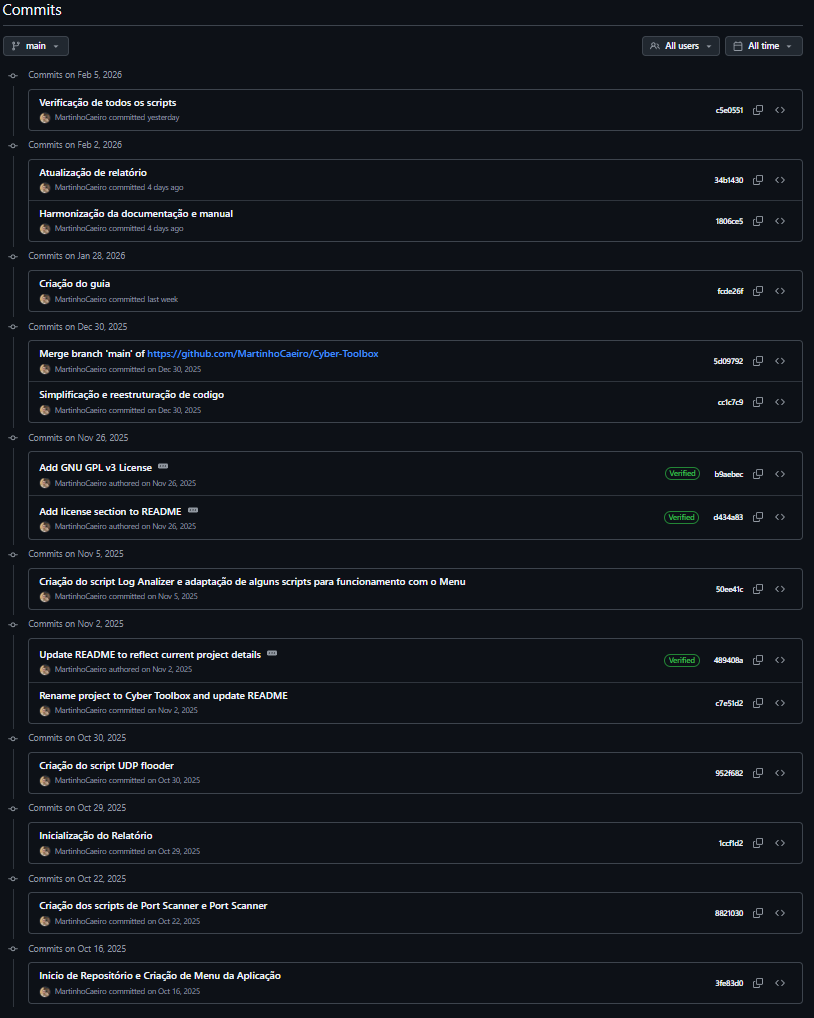
\includegraphics[width=0.7\textwidth]{Recursos/commits.png}
	\caption{Commits no Repositório GitHub}
	\label{fig:nfswarning}
\end{figure}

%---------------------------------------------------------------------------------------------------------------------------
\newpage
\section{Introdução Teórica}\label{theory}
\subsection{Porto}
Um porto (\cite{port}) é um ponto de extremidade lógico para comunicação em rede, usado para identificar serviços ou aplicações específicas em um dispositivo.
Os protocolos que usam principalmente portas são os protocolos da camada de transporte, tais como o Protocolo de controle de transmissão (TCP)
e User Datagram Protocol (UDP) do conjunto de protocolos da internet.

\subsection{UDP Flood}
Um ataque UDP flood (\cite{udpflood}) é um tipo de ataque de negação de serviço (DoS) que visa inundar um alvo com pacotes UDP,
sobrecarregando a largura de banda e os recursos do sistema.

\subsection{SYN Flood}
Um ataque SYN flood (\cite{synflood}) é um tipo de ataque de negação de serviço (DoS) que explora o processo de handshake do TCP,
enviando uma série de pacotes SYN para um servidor, mas nunca completando o handshake, o que pode levar à exaustão dos recursos do mesmo.

\subsection{Logging}
Logging (\cite{logging}) refere-se ao processo de registrar eventos que ocorrem em um sistema de computador.
Esses registos, conhecidos como logs, são essenciais para a análise de segurança,
pois permitem que os administradores identifiquem atividades suspeitas e respondam a incidentes de segurança.

\newpage
\subsection{Port Knocking}
Port Knocking (\cite{portknocking}) é uma técnica de segurança que envolve o envio de uma sequência de pacotes para portas específicas em um servidor,
a fim de abrir uma porta de acesso (geralmente SSH) que está fechada por padrão. Essa técnica é usada para ocultar
serviços de rede e proteger servidores contra ataques automatizados.

\subsection{Password}
Uma password (ou senha) (\cite{password}) é uma sequência de caracteres usada para autenticar a identidade de um utilizador.
As passwords são uma das formas mais comuns de autenticação e são usadas para proteger o acesso a sistemas, contas e dados sensíveis.

\subsection{2FA}
A autenticação de dois fatores (2FA) (\cite{2fa}) é um método de segurança que requer dois tipos diferentes de autenticação para verificar
a identidade de um utilizador. Normalmente, isso envolve algo que o utilizador sabe (como uma password) e algo que o
utilizador possui (como um dispositivo móvel para receber um código temporário).

%---------------------------------------------------------------------------------------------------------------------------
\newpage
\section{Configuração do Servidor}\label{obj}
A instalação do Kali Linux (\cite{kali}), foi feita numa maquina virtual utilizando o VirtualBox (\cite{virtualbox}).
Para facilitar a instalação foi utilizado um .iso feito especificamente para o VirtualBox, que já tinha o processo de instalação
automatizado, poupando assim tempo na instalação do sistema operativo.\\

Informações adicionais incluem 4GB de RAM e seis processadores de CPU e a rede está em modo 'bridge'.
Foi utilizado o Visual Studio Code (\cite{vscode}) como editor de texto para facilitar a edição dos scripts.\\

\begin{figure}[h!]
	\centering
	\includegraphics[width=0.8\textwidth]{Recursos/Server.png}
	\caption{Exemplo de Maquina Utilizada}
	\label{fig:nfswarning}
\end{figure}

%---------------------------------------------------------------------------------------------------------------------------
\newpage
\section{Desenvolvimento dos Scripts}\label{dev}
Todos os seguintes scripts foram desenvolvidos em Python e todos verificam se a maquina possui os pacotes necessários
para o funcionamento da ferramenta, irá perguntar se quer instalar para poder continuar a utilizar. Caso
o utilizador deseje prosseguir, o script irá instalar os pacotes necessários e depois irá ativá-los.
Cada script pode ser executado individualmente ou através do menu principal.

%---------------------------------------------------------------------------------------------------------------------------
\subsection{Menu}
O menu é o metodo principal para a interação com a ferramenta. Para aceder a uma funcionalidade, o utilizador deve selecionar a opção correspondente no menu.
Para executar o menu apenas é necessário escrever `python menu.py`.\\

O menu apresenta-se da seguinte forma:
\begin{figure}[H]
	\centering
	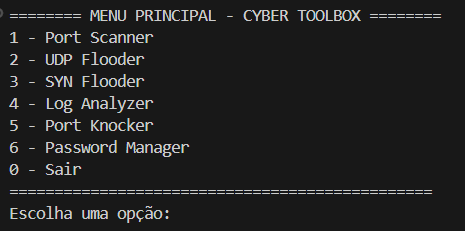
\includegraphics[width=0.9\textwidth]{Recursos/menu.png}
	\caption{Exemplo de execução do Menu Principal}
	\label{fig:menu}
\end{figure}

%---------------------------------------------------------------------------------------------------------------------------
\newpage
\subsection{Port Scanner}

O Port Scanner permite identificar portas TCP abertas em um ou mais alvos. O utilizador indica uma lista de alvos separada por vírgulas e um intervalo de portas (inicial e final). O script resolve cada hostname para IP, testa a conectividade porta a porta com timeout configurável e apresenta os serviços conhecidos quando possível. No final, gera um relatório por alvo com as portas abertas e o tempo total do varrimento. Opcionalmente, pode guardar um relatório em JSON com resultados e métricas, o que facilita a análise posterior.

\begin{figure}[H]
	\centering
	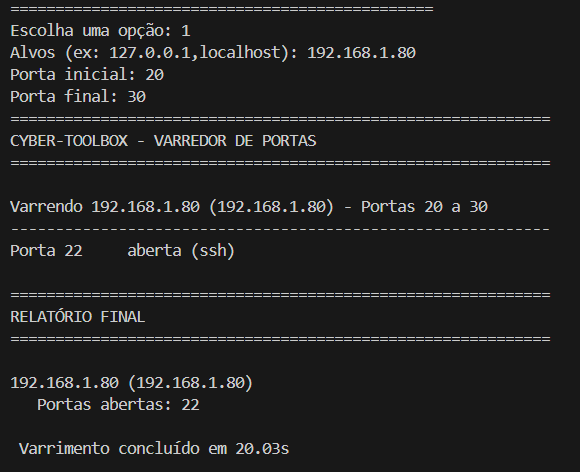
\includegraphics[width=0.9\textwidth]{Recursos/scanner_test.png}
	\caption{Exemplo de execução do Port Scanner}
	\label{fig:scanner_test}
\end{figure}

%---------------------------------------------------------------------------------------------------------------------------
\newpage
\subsection{UDP Flooder}

O UDP Flooder executa um teste de negação de serviço via UDP. O utilizador define o alvo, a porta, a duração, o tamanho do pacote e o número de threads. O script envia pacotes UDP aleatórios de forma concorrente e apresenta estatísticas como total de pacotes enviados e taxa média (pps). Inclui validações de parâmetros e um aviso de segurança com confirmação explícita, reforçando o uso exclusivamente em ambientes autorizados.

\begin{figure}[H]
	\centering
	\begin{subfigure}[b]{0.45\textwidth}
		\centering
		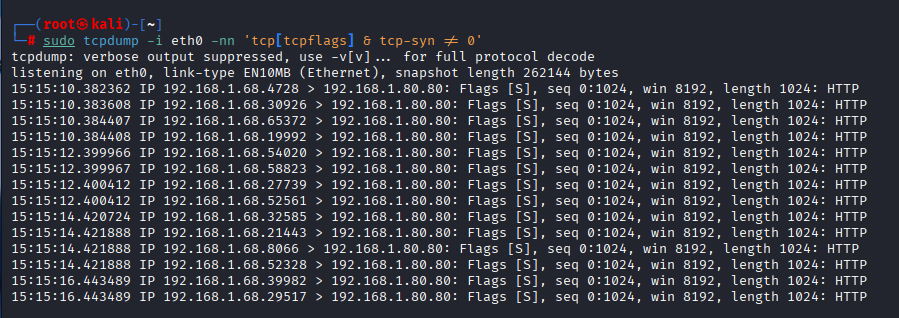
\includegraphics[width=\textwidth]{Recursos/udp_test1.png}
		\caption{Configuração inicial}
		\label{fig:udp_test1}
	\end{subfigure}
	\hfill
	\begin{subfigure}[b]{0.45\textwidth}
		\centering
		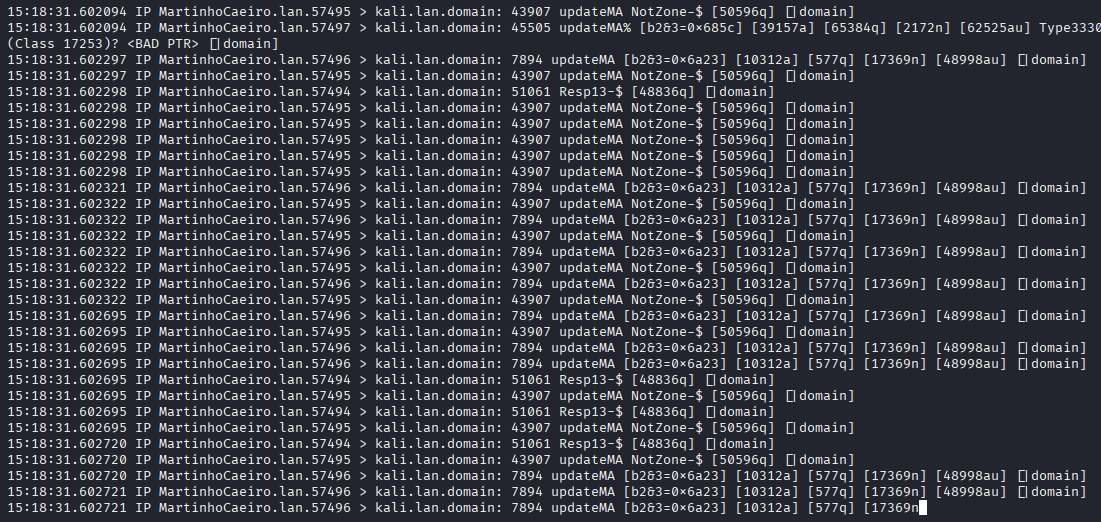
\includegraphics[width=\textwidth]{Recursos/udp_test2.png}
		\caption{Execução do ataque}
		\label{fig:udp_test2}
	\end{subfigure}
	\vskip\baselineskip
	\begin{subfigure}[b]{0.45\textwidth}
		\centering
		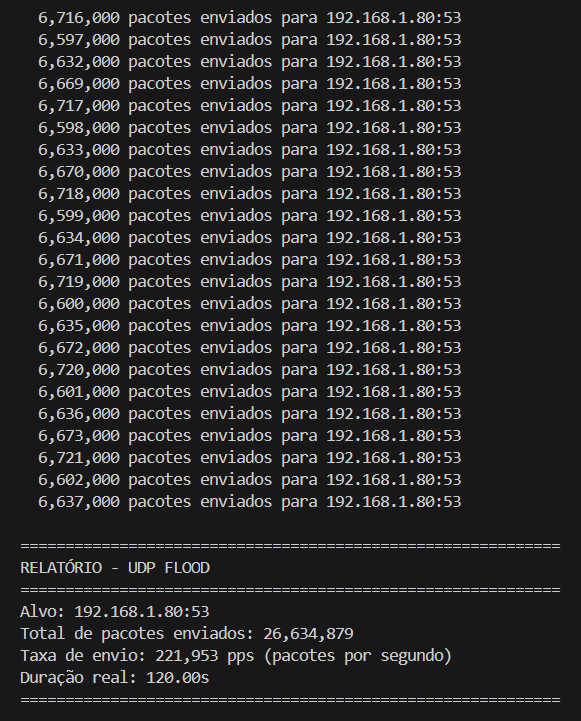
\includegraphics[width=\textwidth]{Recursos/udp_test3.png}
		\caption{Relatório final}
		\label{fig:udp_test3}
	\end{subfigure}
	\caption{Exemplo de execução do UDP Flooder}
	\label{fig:udp_flooder}
\end{figure}

%---------------------------------------------------------------------------------------------------------------------------
\newpage
\subsection{SYN Flooder}

O SYN Flooder simula um ataque DoS baseado em TCP SYN, recorrendo à biblioteca Scapy para criação de pacotes raw. O utilizador indica alvo, porta, duração e threads. Cada thread gera pacotes SYN com IP e porto de origem aleatórios, enviando-os sem completar o handshake. O script mostra progresso e, no fim, apresenta um relatório com número de pacotes e taxa de envio. Requer privilégios de administrador e apresenta um aviso legal antes da execução.

\begin{figure}[H]
	\centering
	\begin{subfigure}[b]{0.6\textwidth}
		\centering
		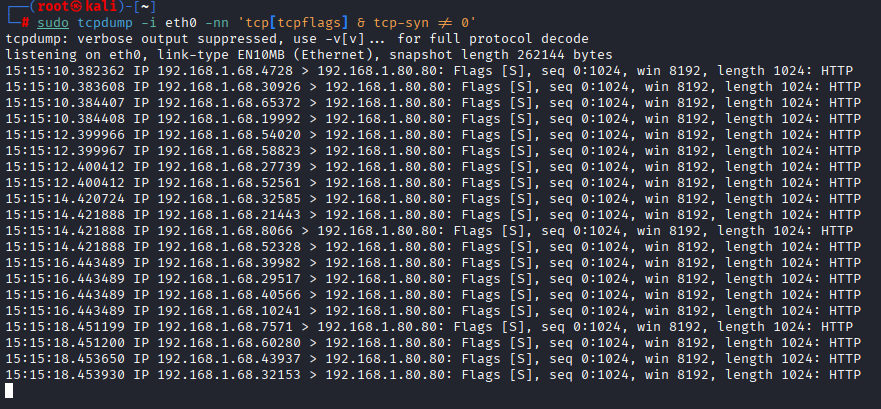
\includegraphics[width=\textwidth]{Recursos/syn_test1.png}
		\caption{Confirmação e início}
		\label{fig:syn_test1}
	\end{subfigure}
	\vskip\baselineskip
	\begin{subfigure}[b]{0.6\textwidth}
		\centering
		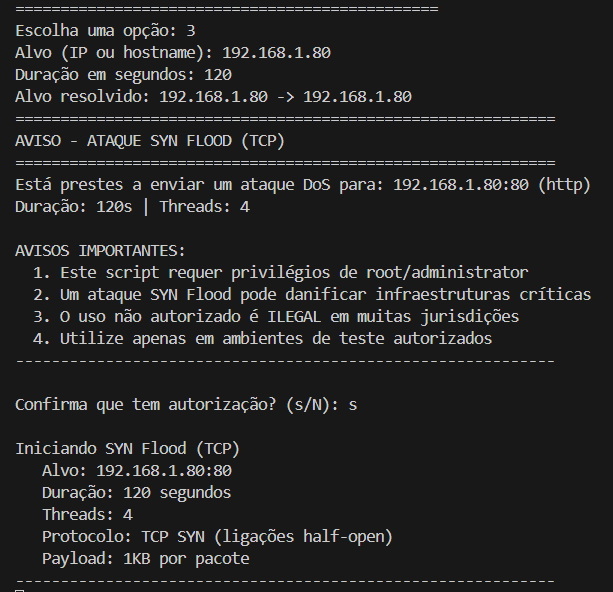
\includegraphics[width=\textwidth]{Recursos/syn_test2.png}
		\caption{Estatísticas finais}
		\label{fig:syn_test2}
	\end{subfigure}
	\caption{Exemplo de execução do SYN Flooder}
	\label{fig:syn_flooder}
\end{figure}

%---------------------------------------------------------------------------------------------------------------------------
\newpage
\subsection{Log Analyzer}

O Log Analyzer analisa ficheiros de logs de servidores web (Apache/Nginx), autenticação SSH e firewall UFW. Utiliza expressões regulares para extrair IP, data/hora, serviço, ação e detalhes relevantes. Quando disponível, integra uma base GeoLite2 para resolver o país de origem dos endereços IP. Para cada ficheiro de entrada, gera relatórios em JSON e CSV e apresenta um resumo com contagens por serviço e top de países. Esta ferramenta é útil para identificar padrões de acesso e eventos suspeitos.

\begin{figure}[H]
	\centering
	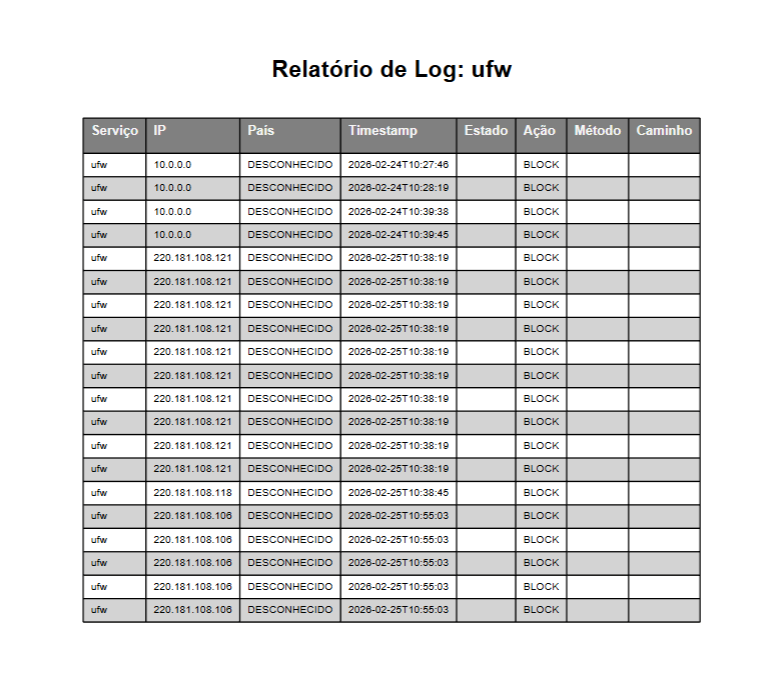
\includegraphics[width=0.9\textwidth]{Recursos/log_test.png}
	\caption{Exemplo de relatório do Log Analyzer}
	\label{fig:log_test}
\end{figure}

%---------------------------------------------------------------------------------------------------------------------------
\newpage
\subsection{Port Knocker}

O Port Knocker envia uma sequência de pacotes UDP para um conjunto de portas específicas, simulando a técnica de port knocking. O utilizador fornece o endereço do servidor e a lista de portas. O script envia um knock por porta com um pequeno atraso entre envios e confirma cada envio. Esta abordagem pode ser usada para abrir serviços ocultos (por exemplo, SSH) apenas após a sequência correta.

\begin{figure}[H]
	\centering
	\begin{subfigure}[b]{0.7\textwidth}
		\centering
		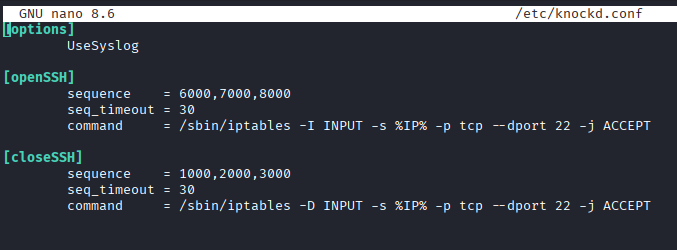
\includegraphics[width=\textwidth]{Recursos/knocker_test1.png}
		\caption{Configuração inicial}
		\label{fig:knocker_test1}
	\end{subfigure}
	\vskip\baselineskip
	\begin{subfigure}[b]{0.7\textwidth}
		\centering
		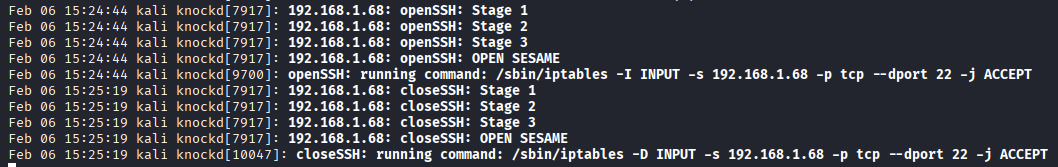
\includegraphics[width=\textwidth]{Recursos/knocker_test2.png}
		\caption{Confirmação de knocks}
		\label{fig:knocker_test2}
	\end{subfigure}
	\vskip\baselineskip
	\begin{subfigure}[b]{0.7\textwidth}
		\centering
		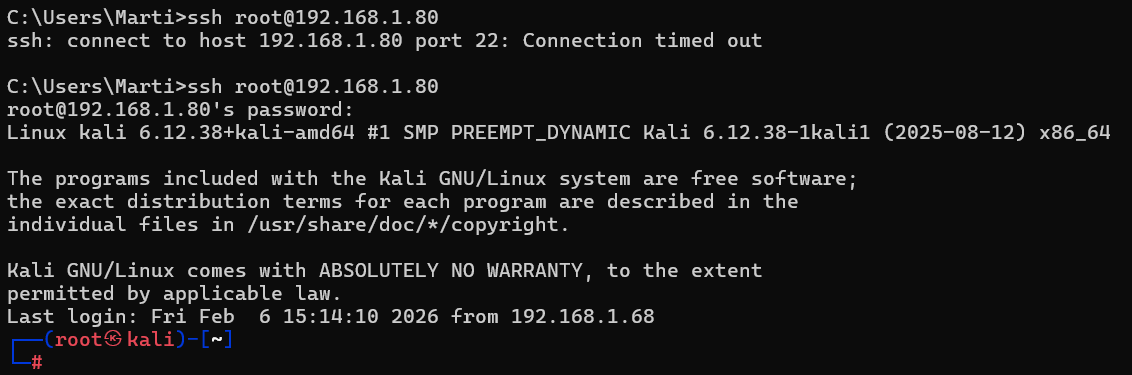
\includegraphics[width=\textwidth]{Recursos/knocker_test3.png}
		\caption{Confirmação de funcionamento}
		\label{fig:knocker_test3}
	\end{subfigure}
	\caption{Exemplo de execução do Port Knocker}
	\label{fig:port_knocker}
\end{figure}

%---------------------------------------------------------------------------------------------------------------------------
\newpage
\subsection{Password Manager}

O Password Manager é um gestor de palavras‑passe com cifragem híbrida (RSA + Fernet) e autenticação de dois fatores via TOTP. O utilizador inicializa o sistema, gerando chaves RSA e um segredo TOTP. Os registos (URL, utilizador e palavra‑passe) são cifrados e guardados numa base local. As operações de listar, ver, atualizar e apagar exigem um código OTP válido, mitigando acessos não autorizados. O script inclui modo não‑interativo e menu interativo, proporcionando flexibilidade de utilização.

\begin{figure}[H]
	\centering
	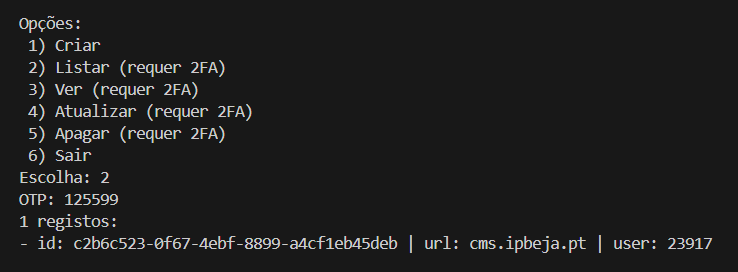
\includegraphics[width=0.9\textwidth]{Recursos/password_test.png}
	\caption{Exemplo de execução do Password Manager}
	\label{fig:password_test}
\end{figure}

%---------------------------------------------------------------------------------------------------------------------------
\newpage
\section{Conclusão}\label{con}
O desenvolvimento deste laboratório permitiu explorar conceitos fundamentais de segurança informática 
e linguagens de programação dinâmicas. Apesar de alguns desafios encontrados, foi possível implementar as 
ferramentas solicitadas e configurar um menu centralizado para facilitar a utilização dos mesmos. 
Durante este processo, foram revistos conceitos previamente estudados, como o Port Knocking, 
e foi dada a oportunidade de aprender novos, como UDP Flooding e SYN Flooding.
%---------------------------------------------------------------------------------------------------------------------------

\newpage
\renewcommand{\refname}{Bibliografia} % Para artigos
\renewcommand{\bibname}{Bibliografia} % Para livros e relatórios
\addcontentsline{toc}{section}{Bibliografia} % Adiciona a Bibliografia ao índice
\printbibliography

\end{document}
